\documentclass{tufte-handout}\usepackage[]{graphicx}\usepackage[]{xcolor}
% maxwidth is the original width if it is less than linewidth
% otherwise use linewidth (to make sure the graphics do not exceed the margin)
\makeatletter
\def\maxwidth{ %
  \ifdim\Gin@nat@width>\linewidth
    \linewidth
  \else
    \Gin@nat@width
  \fi
}
\makeatother

\definecolor{fgcolor}{rgb}{0.345, 0.345, 0.345}
\newcommand{\hlnum}[1]{\textcolor[rgb]{0.686,0.059,0.569}{#1}}%
\newcommand{\hlstr}[1]{\textcolor[rgb]{0.192,0.494,0.8}{#1}}%
\newcommand{\hlcom}[1]{\textcolor[rgb]{0.678,0.584,0.686}{\textit{#1}}}%
\newcommand{\hlopt}[1]{\textcolor[rgb]{0,0,0}{#1}}%
\newcommand{\hlstd}[1]{\textcolor[rgb]{0.345,0.345,0.345}{#1}}%
\newcommand{\hlkwa}[1]{\textcolor[rgb]{0.161,0.373,0.58}{\textbf{#1}}}%
\newcommand{\hlkwb}[1]{\textcolor[rgb]{0.69,0.353,0.396}{#1}}%
\newcommand{\hlkwc}[1]{\textcolor[rgb]{0.333,0.667,0.333}{#1}}%
\newcommand{\hlkwd}[1]{\textcolor[rgb]{0.737,0.353,0.396}{\textbf{#1}}}%
\let\hlipl\hlkwb

\usepackage{framed}
\makeatletter
\newenvironment{kframe}{%
 \def\at@end@of@kframe{}%
 \ifinner\ifhmode%
  \def\at@end@of@kframe{\end{minipage}}%
  \begin{minipage}{\columnwidth}%
 \fi\fi%
 \def\FrameCommand##1{\hskip\@totalleftmargin \hskip-\fboxsep
 \colorbox{shadecolor}{##1}\hskip-\fboxsep
     % There is no \\@totalrightmargin, so:
     \hskip-\linewidth \hskip-\@totalleftmargin \hskip\columnwidth}%
 \MakeFramed {\advance\hsize-\width
   \@totalleftmargin\z@ \linewidth\hsize
   \@setminipage}}%
 {\par\unskip\endMakeFramed%
 \at@end@of@kframe}
\makeatother

\definecolor{shadecolor}{rgb}{.97, .97, .97}
\definecolor{messagecolor}{rgb}{0, 0, 0}
\definecolor{warningcolor}{rgb}{1, 0, 1}
\definecolor{errorcolor}{rgb}{1, 0, 0}
\newenvironment{knitrout}{}{} % an empty environment to be redefined in TeX

\usepackage{alltt}

\title{Reaction Kinetics for Air Pollution}
% \date{}
\IfFileExists{upquote.sty}{\usepackage{upquote}}{}
\begin{document}

\maketitle


Here's an example R code for simulating reaction kinetics in the context of air pollution using a simple chemical reaction model. In this example, I'll use the well-known reaction of pollutants A and B reacting to form a product C. This is a simplified model, and the actual chemical reactions in the atmosphere can be more complex.

\begin{knitrout}
\definecolor{shadecolor}{rgb}{0.969, 0.969, 0.969}\color{fgcolor}\begin{kframe}
\begin{alltt}
\hlcom{# Reaction Kinetics for Air Pollution}

\hlcom{# Parameters}
\hlstd{rate_constant} \hlkwb{<-} \hlnum{0.01}   \hlcom{# Reaction rate constant}
\hlstd{initial_concentration_A} \hlkwb{<-} \hlnum{1.0}  \hlcom{# Initial concentration of pollutant A}
\hlstd{initial_concentration_B} \hlkwb{<-} \hlnum{0.5}  \hlcom{# Initial concentration of pollutant B}
\hlstd{initial_concentration_C} \hlkwb{<-} \hlnum{0.0}  \hlcom{# Initial concentration of product C}

\hlcom{# Simulation parameters}
\hlstd{dt} \hlkwb{<-} \hlnum{0.1}    \hlcom{# Time step}
\hlstd{num_steps} \hlkwb{<-} \hlnum{100}   \hlcom{# Number of time steps}

\hlcom{# Initialize concentrations}
\hlstd{concentration_A} \hlkwb{<-} \hlkwd{rep}\hlstd{(}\hlnum{0}\hlstd{, num_steps)}
\hlstd{concentration_B} \hlkwb{<-} \hlkwd{rep}\hlstd{(}\hlnum{0}\hlstd{, num_steps)}
\hlstd{concentration_C} \hlkwb{<-} \hlkwd{rep}\hlstd{(}\hlnum{0}\hlstd{, num_steps)}

\hlstd{concentration_A[}\hlnum{1}\hlstd{]} \hlkwb{<-} \hlstd{initial_concentration_A}
\hlstd{concentration_B[}\hlnum{1}\hlstd{]} \hlkwb{<-} \hlstd{initial_concentration_B}
\hlstd{concentration_C[}\hlnum{1}\hlstd{]} \hlkwb{<-} \hlstd{initial_concentration_C}

\hlcom{# Reaction kinetics simulation loop}
\hlkwa{for} \hlstd{(step} \hlkwa{in} \hlnum{2}\hlopt{:}\hlstd{num_steps) \{}
  \hlcom{# Reaction kinetics}
  \hlstd{dA_dt} \hlkwb{<-} \hlopt{-}\hlstd{rate_constant} \hlopt{*} \hlstd{concentration_A[step} \hlopt{-} \hlnum{1}\hlstd{]} \hlopt{*} \hlstd{concentration_B[step} \hlopt{-} \hlnum{1}\hlstd{]} \hlopt{*} \hlstd{dt}
  \hlstd{dB_dt} \hlkwb{<-} \hlopt{-}\hlstd{rate_constant} \hlopt{*} \hlstd{concentration_A[step} \hlopt{-} \hlnum{1}\hlstd{]} \hlopt{*} \hlstd{concentration_B[step} \hlopt{-} \hlnum{1}\hlstd{]} \hlopt{*} \hlstd{dt}
  \hlstd{dC_dt} \hlkwb{<-} \hlstd{rate_constant} \hlopt{*} \hlstd{concentration_A[step} \hlopt{-} \hlnum{1}\hlstd{]} \hlopt{*} \hlstd{concentration_B[step} \hlopt{-} \hlnum{1}\hlstd{]} \hlopt{*} \hlstd{dt}

  \hlcom{# Update concentrations}
  \hlstd{concentration_A[step]} \hlkwb{<-} \hlstd{concentration_A[step} \hlopt{-} \hlnum{1}\hlstd{]} \hlopt{+} \hlstd{dA_dt}
  \hlstd{concentration_B[step]} \hlkwb{<-} \hlstd{concentration_B[step} \hlopt{-} \hlnum{1}\hlstd{]} \hlopt{+} \hlstd{dB_dt}
  \hlstd{concentration_C[step]} \hlkwb{<-} \hlstd{concentration_C[step} \hlopt{-} \hlnum{1}\hlstd{]} \hlopt{+} \hlstd{dC_dt}
\hlstd{\}}

\hlcom{# Plotting the results}
\hlstd{time} \hlkwb{<-} \hlkwd{seq}\hlstd{(}\hlnum{0}\hlstd{, (num_steps} \hlopt{-} \hlnum{1}\hlstd{)} \hlopt{*} \hlstd{dt,} \hlkwc{by} \hlstd{= dt)}

\hlkwd{plot}\hlstd{(time, concentration_A,} \hlkwc{type} \hlstd{=} \hlstr{'l'}\hlstd{,} \hlkwc{col} \hlstd{=} \hlstr{'red'}\hlstd{,} \hlkwc{lwd} \hlstd{=} \hlnum{2}\hlstd{,} \hlkwc{ylim} \hlstd{=} \hlkwd{c}\hlstd{(}\hlnum{0}\hlstd{,} \hlkwd{max}\hlstd{(initial_concentration_A, initial_concentration_B, initial_concentration_C)))}
\hlkwd{lines}\hlstd{(time, concentration_B,} \hlkwc{type} \hlstd{=} \hlstr{'l'}\hlstd{,} \hlkwc{col} \hlstd{=} \hlstr{'blue'}\hlstd{,} \hlkwc{lwd} \hlstd{=} \hlnum{2}\hlstd{)}
\hlkwd{lines}\hlstd{(time, concentration_C,} \hlkwc{type} \hlstd{=} \hlstr{'l'}\hlstd{,} \hlkwc{col} \hlstd{=} \hlstr{'green'}\hlstd{,} \hlkwc{lwd} \hlstd{=} \hlnum{2}\hlstd{)}

\hlkwd{legend}\hlstd{(}\hlstr{'topright'}\hlstd{,} \hlkwc{legend} \hlstd{=} \hlkwd{c}\hlstd{(}\hlstr{'A'}\hlstd{,} \hlstr{'B'}\hlstd{,} \hlstr{'C'}\hlstd{),} \hlkwc{col} \hlstd{=} \hlkwd{c}\hlstd{(}\hlstr{'red'}\hlstd{,} \hlstr{'blue'}\hlstd{,} \hlstr{'green'}\hlstd{),} \hlkwc{lwd} \hlstd{=} \hlnum{2}\hlstd{,} \hlkwc{bty} \hlstd{=} \hlstr{'n'}\hlstd{)}
\hlkwd{title}\hlstd{(}\hlkwc{main} \hlstd{=} \hlstr{'Reaction Kinetics for Air Pollution'}\hlstd{)}
\hlstd{xlabel} \hlkwb{<-} \hlkwd{expression}\hlstd{(}\hlstr{'Time ('} \hlopt{~} \hlstd{s} \hlopt{~} \hlstr{')'}\hlstd{)}
\hlstd{ylabel} \hlkwb{<-} \hlkwd{expression}\hlstd{(}\hlstr{'Concentration'}\hlstd{)}
\hlkwd{title}\hlstd{(}\hlkwc{xlab} \hlstd{= xlabel,} \hlkwc{ylab} \hlstd{= ylabel)}
\end{alltt}
\end{kframe}
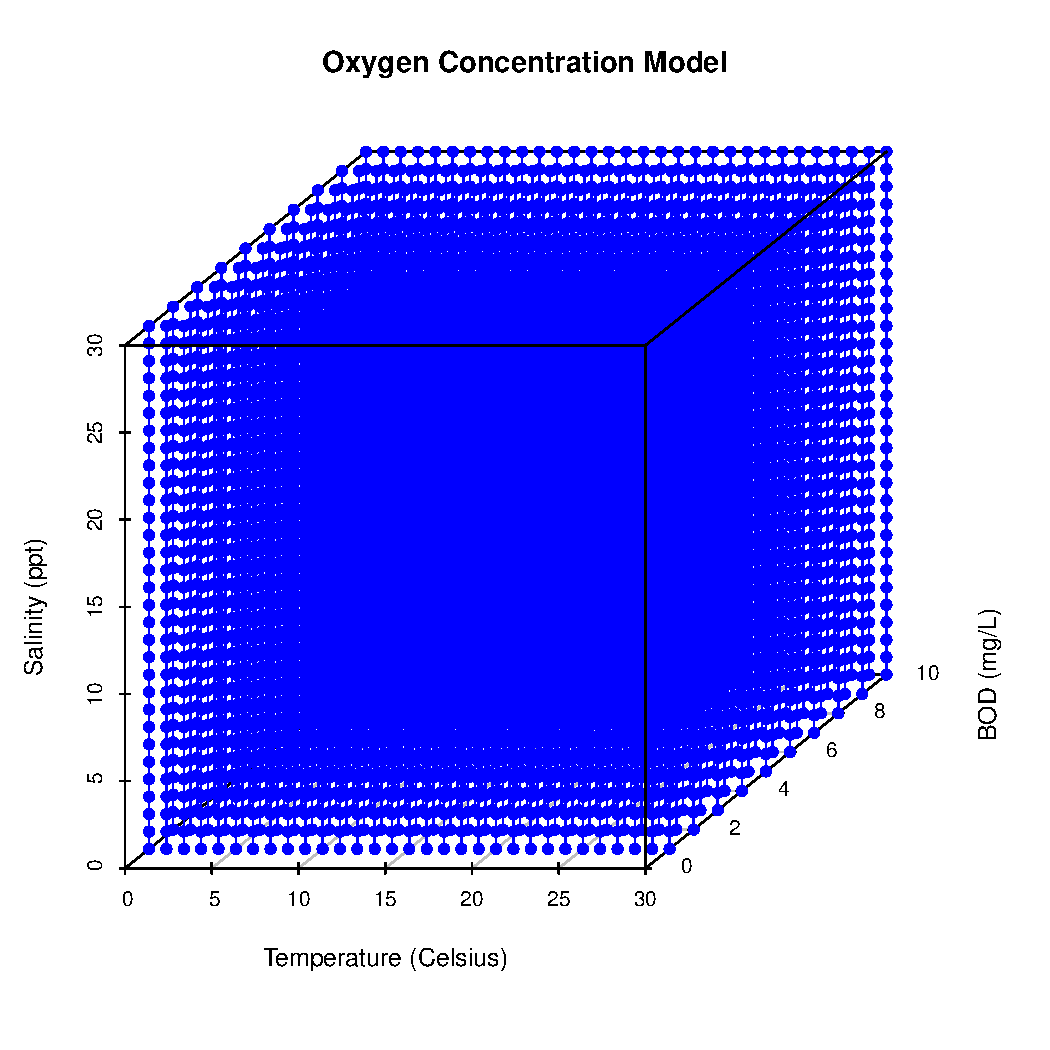
\includegraphics[width=\maxwidth]{figure/unnamed-chunk-1-1} 
\end{knitrout}


\section{with temperature}
\begin{knitrout}
\definecolor{shadecolor}{rgb}{0.969, 0.969, 0.969}\color{fgcolor}\begin{kframe}
\begin{alltt}
\hlcom{# Reaction Kinetics for Air Pollution with Temperature}

\hlcom{# Parameters}
\hlstd{initial_concentration_A} \hlkwb{<-} \hlnum{1.0}  \hlcom{# Initial concentration of pollutant A}
\hlstd{initial_concentration_B} \hlkwb{<-} \hlnum{0.5}  \hlcom{# Initial concentration of pollutant B}
\hlstd{initial_concentration_C} \hlkwb{<-} \hlnum{0.0}  \hlcom{# Initial concentration of product C}

\hlcom{# Simulation parameters}
\hlstd{dt} \hlkwb{<-} \hlnum{0.1}    \hlcom{# Time step}
\hlstd{num_steps} \hlkwb{<-} \hlnum{100}   \hlcom{# Number of time steps}

\hlcom{# Temperature parameters}
\hlstd{initial_temperature} \hlkwb{<-} \hlnum{300}  \hlcom{# Initial temperature in Kelvin}
\hlstd{temperature_increase_rate} \hlkwb{<-} \hlnum{1}  \hlcom{# Rate of temperature increase over time}
\hlstd{activation_energy} \hlkwb{<-} \hlnum{20}  \hlcom{# Activation energy for the reaction}

\hlcom{# Function to calculate the rate constant based on temperature}
\hlstd{calculate_rate_constant} \hlkwb{<-} \hlkwa{function}\hlstd{(}\hlkwc{temperature}\hlstd{) \{}
  \hlkwd{return}\hlstd{(}\hlkwd{exp}\hlstd{(}\hlopt{-}\hlstd{activation_energy} \hlopt{/} \hlstd{(}\hlnum{8.314} \hlopt{*} \hlstd{temperature)))}
\hlstd{\}}

\hlcom{# Initialize concentrations and temperature}
\hlstd{concentration_A} \hlkwb{<-} \hlkwd{rep}\hlstd{(}\hlnum{0}\hlstd{, num_steps)}
\hlstd{concentration_B} \hlkwb{<-} \hlkwd{rep}\hlstd{(}\hlnum{0}\hlstd{, num_steps)}
\hlstd{concentration_C} \hlkwb{<-} \hlkwd{rep}\hlstd{(}\hlnum{0}\hlstd{, num_steps)}
\hlstd{temperature} \hlkwb{<-} \hlkwd{rep}\hlstd{(}\hlnum{0}\hlstd{, num_steps)}

\hlstd{concentration_A[}\hlnum{1}\hlstd{]} \hlkwb{<-} \hlstd{initial_concentration_A}
\hlstd{concentration_B[}\hlnum{1}\hlstd{]} \hlkwb{<-} \hlstd{initial_concentration_B}
\hlstd{concentration_C[}\hlnum{1}\hlstd{]} \hlkwb{<-} \hlstd{initial_concentration_C}
\hlstd{temperature[}\hlnum{1}\hlstd{]} \hlkwb{<-} \hlstd{initial_temperature}

\hlcom{# Reaction kinetics simulation loop}
\hlkwa{for} \hlstd{(step} \hlkwa{in} \hlnum{2}\hlopt{:}\hlstd{num_steps) \{}
  \hlcom{# Temperature increase over time}
  \hlstd{temperature[step]} \hlkwb{<-} \hlstd{initial_temperature} \hlopt{+} \hlstd{temperature_increase_rate} \hlopt{*} \hlstd{(step} \hlopt{-} \hlnum{1}\hlstd{)} \hlopt{*} \hlstd{dt}

  \hlcom{# Reaction kinetics with temperature dependence}
  \hlstd{rate_constant} \hlkwb{<-} \hlkwd{calculate_rate_constant}\hlstd{(temperature[step])}

  \hlstd{dA_dt} \hlkwb{<-} \hlopt{-}\hlstd{rate_constant} \hlopt{*} \hlstd{concentration_A[step} \hlopt{-} \hlnum{1}\hlstd{]} \hlopt{*} \hlstd{concentration_B[step} \hlopt{-} \hlnum{1}\hlstd{]} \hlopt{*} \hlstd{dt}
  \hlstd{dB_dt} \hlkwb{<-} \hlopt{-}\hlstd{rate_constant} \hlopt{*} \hlstd{concentration_A[step} \hlopt{-} \hlnum{1}\hlstd{]} \hlopt{*} \hlstd{concentration_B[step} \hlopt{-} \hlnum{1}\hlstd{]} \hlopt{*} \hlstd{dt}
  \hlstd{dC_dt} \hlkwb{<-} \hlstd{rate_constant} \hlopt{*} \hlstd{concentration_A[step} \hlopt{-} \hlnum{1}\hlstd{]} \hlopt{*} \hlstd{concentration_B[step} \hlopt{-} \hlnum{1}\hlstd{]} \hlopt{*} \hlstd{dt}

  \hlcom{# Update concentrations}
  \hlstd{concentration_A[step]} \hlkwb{<-} \hlstd{concentration_A[step} \hlopt{-} \hlnum{1}\hlstd{]} \hlopt{+} \hlstd{dA_dt}
  \hlstd{concentration_B[step]} \hlkwb{<-} \hlstd{concentration_B[step} \hlopt{-} \hlnum{1}\hlstd{]} \hlopt{+} \hlstd{dB_dt}
  \hlstd{concentration_C[step]} \hlkwb{<-} \hlstd{concentration_C[step} \hlopt{-} \hlnum{1}\hlstd{]} \hlopt{+} \hlstd{dC_dt}
\hlstd{\}}

\hlcom{# Plotting the results}
\hlstd{time} \hlkwb{<-} \hlkwd{seq}\hlstd{(}\hlnum{0}\hlstd{, (num_steps} \hlopt{-} \hlnum{1}\hlstd{)} \hlopt{*} \hlstd{dt,} \hlkwc{by} \hlstd{= dt)}

\hlkwd{par}\hlstd{(}\hlkwc{mfrow} \hlstd{=} \hlkwd{c}\hlstd{(}\hlnum{2}\hlstd{,} \hlnum{1}\hlstd{),} \hlkwc{mar} \hlstd{=} \hlkwd{c}\hlstd{(}\hlnum{4}\hlstd{,} \hlnum{4}\hlstd{,} \hlnum{2}\hlstd{,} \hlnum{2}\hlstd{),} \hlkwc{oma} \hlstd{=} \hlkwd{c}\hlstd{(}\hlnum{0}\hlstd{,} \hlnum{0}\hlstd{,} \hlnum{2}\hlstd{,} \hlnum{0}\hlstd{))}
\hlkwd{plot}\hlstd{(time, concentration_A,} \hlkwc{type} \hlstd{=} \hlstr{'l'}\hlstd{,} \hlkwc{col} \hlstd{=} \hlstr{'red'}\hlstd{,} \hlkwc{lwd} \hlstd{=} \hlnum{2}\hlstd{,} \hlkwc{ylim} \hlstd{=} \hlkwd{c}\hlstd{(}\hlnum{0}\hlstd{,} \hlkwd{max}\hlstd{(initial_concentration_A, initial_concentration_B, initial_concentration_C)))}
\hlkwd{lines}\hlstd{(time, concentration_B,} \hlkwc{type} \hlstd{=} \hlstr{'l'}\hlstd{,} \hlkwc{col} \hlstd{=} \hlstr{'blue'}\hlstd{,} \hlkwc{lwd} \hlstd{=} \hlnum{2}\hlstd{)}
\hlkwd{lines}\hlstd{(time, concentration_C,} \hlkwc{type} \hlstd{=} \hlstr{'l'}\hlstd{,} \hlkwc{col} \hlstd{=} \hlstr{'green'}\hlstd{,} \hlkwc{lwd} \hlstd{=} \hlnum{2}\hlstd{)}
\hlkwd{legend}\hlstd{(}\hlstr{'topright'}\hlstd{,} \hlkwc{legend} \hlstd{=} \hlkwd{c}\hlstd{(}\hlstr{'A'}\hlstd{,} \hlstr{'B'}\hlstd{,} \hlstr{'C'}\hlstd{),} \hlkwc{col} \hlstd{=} \hlkwd{c}\hlstd{(}\hlstr{'red'}\hlstd{,} \hlstr{'blue'}\hlstd{,} \hlstr{'green'}\hlstd{),} \hlkwc{lwd} \hlstd{=} \hlnum{2}\hlstd{,} \hlkwc{bty} \hlstd{=} \hlstr{'n'}\hlstd{)}
\hlkwd{title}\hlstd{(}\hlkwc{main} \hlstd{=} \hlstr{'Reaction Kinetics for Air Pollution'}\hlstd{)}

\hlkwd{plot}\hlstd{(time, temperature,} \hlkwc{type} \hlstd{=} \hlstr{'l'}\hlstd{,} \hlkwc{col} \hlstd{=} \hlstr{'orange'}\hlstd{,} \hlkwc{lwd} \hlstd{=} \hlnum{2}\hlstd{,} \hlkwc{ylim} \hlstd{=} \hlkwd{c}\hlstd{(initial_temperature,} \hlkwd{max}\hlstd{(temperature)))}
\hlkwd{title}\hlstd{(}\hlkwc{main} \hlstd{=} \hlstr{'Temperature Profile'}\hlstd{)}
\hlstd{xlabel} \hlkwb{<-} \hlkwd{expression}\hlstd{(}\hlstr{'Time ('} \hlopt{~} \hlstd{s} \hlopt{~} \hlstr{')'}\hlstd{)}
\hlstd{ylabel} \hlkwb{<-} \hlkwd{expression}\hlstd{(}\hlstr{'Temperature (K)'}\hlstd{)}
\hlkwd{title}\hlstd{(}\hlkwc{xlab} \hlstd{= xlabel,} \hlkwc{ylab} \hlstd{= ylabel)}
\end{alltt}
\end{kframe}
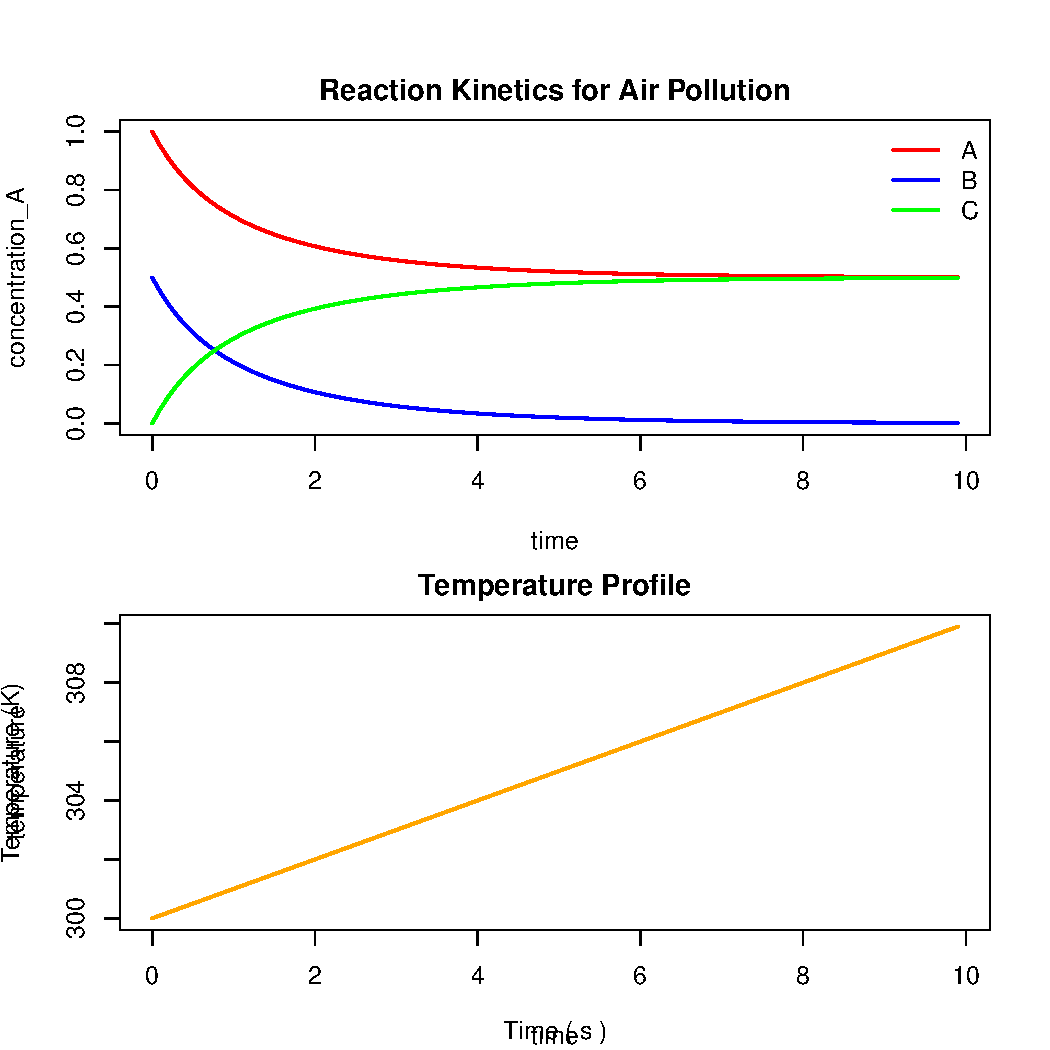
\includegraphics[width=\maxwidth]{figure/unnamed-chunk-2-1} 
\end{knitrout}

\end{document}
